\chapter{Einleitung}
\label{chap:einleitung}

In der heutigen Industrie 4.0 spielen \textbf{Embedded Systems und Edge-Computing} eine zentrale Rolle in der 
Automatisierung und Optimierung von Produktionsprozessen. Diese Technologien ermöglichen es, Maschinen 
und Produktionssysteme mit Intelligenz auszustatten. Die Daten werden direkt an der Quelle verarbeiten 
um schnelle und datengesteuerte Entscheidungen zu treffen. Besonders im industriellen Umfeld, wo Ressourcen 
wie Speicher und Rechenleistung oft begrenzt sind, bietet der Einsatz von \ML auf Embedded Systemen 
eine vielversprechende, aber zugleich herausfordernde Möglichkeit.

Die Relevanz von \ML in der Industrie steht außer Frage. Von der \textbf{vorausschauenden Wartung} \cite{inbook} 
bis hin zur \textbf{Qualitätskontrolle} \cite{phdthesis} bietet \ML zahlreiche Möglichkeiten zur Effizienzsteigerung und 
Kostensenkung. Allerdings sind viele bestehende Machine-Learning-Modelle nicht für den Einsatz auf Embedded Systemen 
optimiert \cite{article}. Die besonderen Herausforderungen, die sich durch eingeschränkte Ressourcen und strenge 
Echtzeitanforderungen ergeben, erfordern spezialisierte Ansätze für das Modell-Deployment auf solchen 
Systemen.

Aktuelle Forschung zeigt, dass der Einsatz von Machine Learning in Embedded Systemen zunehmend an 
Bedeutung gewinnt \cite{s23042131}. Zahlreiche Studien betonen die Vorteile von Edge-Computing in 
industriellen Anwendungen, insbesondere im Hinblick auf \textbf{Echtzeitanalysen und datengesteuerte 
Entscheidungsprozesse} \cite{10212294}. Diese Arbeit knüpft an diese Forschung an und 
erweitert sie, indem ein Framework entwickelt wird, das speziell auf die Herausforderungen im 
industriellen Umfeld zugeschnitten ist.

Das Hauptziel dieser Arbeit ist es, ein optimiertes Modell-Deployment auf Embedded Systemen zu 
realisieren, das den spezifischen Bedingungen in der industriellen Umgebung gerecht wird. Dabei 
werden sowohl die technischen Herausforderungen als auch die praktischen Implikationen des Einsatzes 
von \ML auf speicher- und rechenleistungseingeschränkten Systemen untersucht.
\begin{figure}[h] 
    \centering
    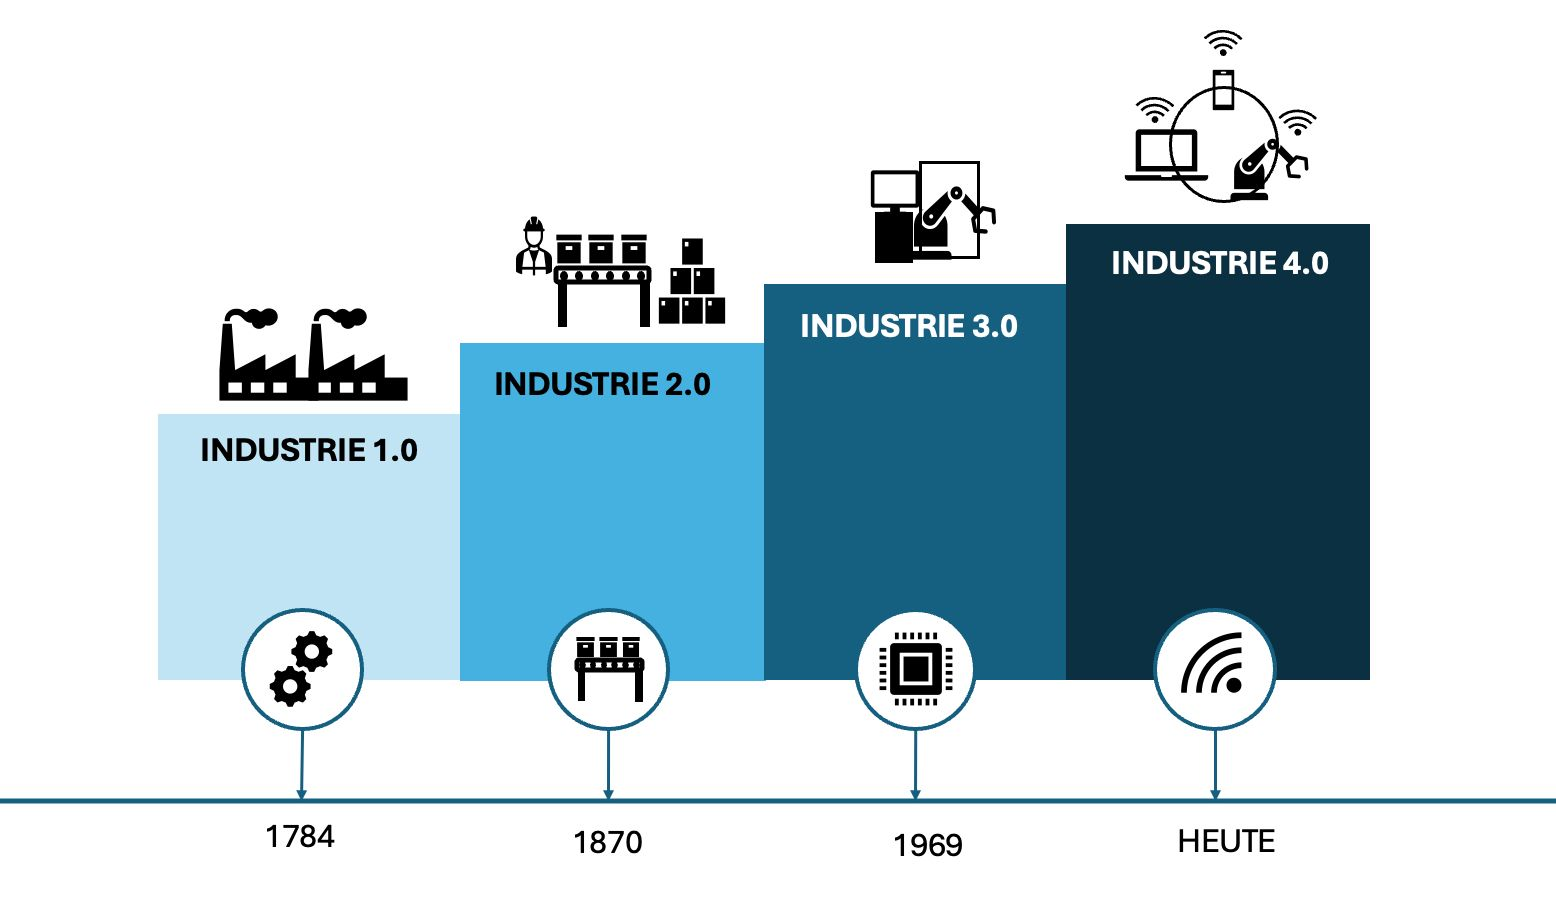
\includegraphics[width=1\textwidth]{IndustrieVierNull.jpeg} 
    \caption{Die vier industriellen Revolutionen: Mechanisierung, Massenproduktion, Automatisierung, Vernetzte Systeme.}
    \label{fig:industrie_vier_null}
\end{figure}
Die Innovation dieser Arbeit liegt in der Entwicklung eines \textbf{optimierten Frameworks}, das sowohl die 
spezifischen Hardware-Einschränkungen von Embedded Systemen als auch die strengen Echtzeitanforderungen 
im industriellen Kontext berücksichtigt. Während bestehende Ansätze oft allgemeine Lösungen bieten, 
konzentriert sich dieses Framework auf die besonderen Herausforderungen in speicher- und 
rechenleistungseingeschränkten Umgebungen.

Ein spezifisch angepasstes ML-Framework zur Bereitstellung und Optimierung von ML-Modellen auf Embedded Systemen 
ist in der industriellen Praxis von hoher Relevanz. Der Entwurf eines ML-Frameworks, das die Anforderungen von 
Embedded Systemen in der Fertigung erfüllt, erfordert eine genaue Analyse der Hardwarebeschränkungen und die 
Implementierung \textbf{effizienter Algorithmen}, die bei begrenzter Rechenkapazität eine hohe Modellgenauigkeit bieten. 
Ein entscheidender Vorteil des Edge-Computings liegt in der lokalen Datenverarbeitung, die Latenzzeiten reduziert 
und gleichzeitig die Sicherheit und Vertraulichkeit der Daten erhöht. Durch die Entwicklung eines solchen 
Frameworks könnte diese Arbeit dazu beitragen, Embedded Systeme besser für den Einsatz von ML-Anwendungen nutzbar 
zu machen und so die Produktionsprozesse zu verbessern.

Um dieses Ziel zu erreichen, kombiniert diese Arbeit eine strukturierte Literaturrecherche sowie eine 
praxisnahe Anforderungsanalyse. Zunächst werden die theoretischen Grundlagen von Embedded Systems und 
Machine Learning in der Industrie 4.0 untersucht. Anschließend entsteht ein Framework, das speziell auf 
die Anforderungen von Embedded Systemen abgestimmt ist. Dieses Framework wird in einer industriellen 
Umgebung getestet, um seine Leistungsfähigkeit und Effizienz zu validieren. Dabei sollen folgende 
Forschungsfragen beantwortet werden: 

\begin{quote}
    \textbf{Forschungsfragen:}
    \begin{enumerate}
        \item Wie kann ein ML-Framework für Embedded Systeme optimiert werden, um den Anforderungen der Industrie 4.0 zu entsprechen?
        \item Welche spezifischen Anpassungen sind für ressourcenbeschränkte Umgebungen notwendig?
    \end{enumerate}
\end{quote}

Die Arbeit ist wie folgt strukturiert: In Kapitel \ref{chap:theoretische_hintergrund} werden die 
theoretischen Grundlagen und der Stand der Technik im Bereich Embedded Systems und Machine Learning 
in der Industrie 4.0 erörtert. Kapitel \ref{chap:methodik} beschreibt die Methodik, die bei der 
Entwicklung des Frameworks angewendet wird. In Kapitel \ref{chap:entwicklung_framework} wird das 
entwickelte Framework im Detail vorgestellt, gefolgt von der Implementierung und Optimierung in 
Kapitel \ref{chap:implementierung_optimierung}. Die Evaluation des Frameworks erfolgt in Kapitel 
\ref{chap:evaluation}, bevor in Kapitel \ref{chap:diskussion} die Ergebnisse diskutiert werden. 
Abschließend fasst Kapitel \ref{chap:fazit} die Arbeit zusammen und gibt einen Ausblick auf 
zukünftige Entwicklungen.